\documentclass[12pt,a4paper]{report}

\usepackage[english,russian]{babel}
\usepackage[T2A]{fontenc}
\usepackage[utf8]{inputenc}
\usepackage{amsmath}
\usepackage{amsfonts}
\usepackage{amssymb}
\usepackage{graphicx}
\usepackage{listings}

\voffset -24.5mm
\hoffset -5mm
\textwidth 173mm
\textheight 240mm
\oddsidemargin=0mm \evensidemargin=0mm

\lstdefinestyle{CppCodeStyle}{
	basicstyle=\footnotesize\ttfamily,
	language={[ANSI]C++},
	keywordstyle=\bfseries,
	showstringspaces=false,
	morekeywords={include, printf},
	commentstyle={},
	texcl=true,
	frame=single,
	breaklines=true,
	extendedchars=\true
}

\begin{document}
	\begin{titlepage}
\begin{center}

\textbf{Санкт-Петербургский политехнический университет Петра Великого}

\vspace{5mm}
Институт компьютерных наук и технологий

\vspace{5mm}
Кафедра компьютерных систем и программных технологий

\vspace*{\fill}

\Large{\textbf{Отчет по лабораторной работе №1}}

\large{по дисциплине: <<Параллельные вычисления>>}

\vspace*{2mm}
\large{Тема работы: <<Определение частоты встречи слов в тексте на русском языке>>}

\vspace*{\fill}
\end{center}

%\begin{flushright}
\begin{large}
\hspace{0.4\linewidth} \textbf{Работу выполнила}

\vspace{5mm}
\hspace{0.4\linewidth} студентка группы 13541/3

\vspace{3mm}
\hspace{0.4\linewidth} \underline{\hspace{2cm} } \hspace{3mm} Мартюшева Н. Ю.

\vspace{3mm}
\hspace{0.4\linewidth} \textbf{Преподаватель}

\vspace{5mm}
\hspace{0.4\linewidth} \underline{\hspace{2cm} } \hspace{3mm} Стручков И.В.
\end{large}
%\end{flushright}

\vspace*{3cm}

\begin{center}
\normalsize Санкт-Петербург\\2018
\end{center}
\end{titlepage}
	
	\renewcommand{\thesection}{\arabic{section}}
	\tableofcontents
	\pagebreak
	
	\setcounter{totalnumber}{10}
	\setcounter{topnumber}{10}
	\setcounter{bottomnumber}{10}
	\renewcommand{\topfraction}{1}
	\renewcommand{\textfraction}{0}
	
	\section{Постановка задачи}
		В рамках лабораторной работы необходимо реализовать программу, определяющую частоту встречи слов в тексте на русском языке. 
		
		Программа должна быть разработана в следующих вариантах:
		\begin{enumerate}
			\item Параллельная реализация при помощи POSIX threads;
			\item Параллельная реализация при помощи технологии MPI.
		\end{enumerate}
		
		Необходимо произвести оценку скорости работы различных вариантов программы в зависимости от окружения, а так же от количества потоков (процессов).
		
	\section{Реализация}
		Опишем входные параметры, алгоритм работы и формат результата каждого варианта программы.
				
		\subsection{Параллельная реализация при помощи POSIX threads}
			В качестве параметров программе передается количество потоков и имя файла с текстом на русском языке. Результатом работы программы является сообщение в следующем формате: в первой строке вывода записано \textit{время выполнения программы в миллисекундах}, затем построчно выводится информация о количестве повторений слов в формате \textit{"Слово Количество\_повторений"}.
					
			Программа работает по следующему алгоритму:
				\begin{enumerate}
					\item Инициализируем глобальные переменные: вектор для хранения слов, map для хранения повторений слов, мьютекс для обеспечения совместного доступа к глобальным переменным.
					\item Получаем из параметра количество потоков (N).
					\item Получаем из параметра имя файла.
					\item Открываем файловый поток и получаем информацию о размере анализируемого файла (size), размере части файла для анализа в одном потоке (size/N).
					\item Считываем входной файл в массив типа char.
					\item Инициализируем таймер и получаем время начала работы программы.
					\item Разбиваем входной массив на N массивов примерно одинаковой длинны (size/N). Для этого из входной строки берем подстроку длиной size/N, а затем смещаем границу до первого разделяющего символа (пробела, точки, запятой и т.д.). Таким образов формируется рабочий массив для каждого потока.
					\item Запускаем функцию подсчета количества слов для каждого из N потоков, передав ему соответствующую подстроку:
						\begin{enumerate}
							\item Инициализируем локальные вектор и карту для подсчета слов.
							\item Последовательно анализируем каждое слово в подстроке, до тех пор, пока не закончится строка:
							\begin{itemize}
								\item Если слова нет в векторе встреченных слов, то добавляем его и в вектор \textit{Новое\_слово}, и в map в виде пары \textit{Новое\_слово 1}.
								\item Если слово есть в векторе встреченных слов, то увеличиваем соответствующее значение в map на 1.
							\end{itemize}
							\item Переводим мьютекс в заблокированное состояние.
							\item Объединяем локальные вектор и карту с глобальными вектором и картой.
							\item Разблокируем мьютекс.
						\end{enumerate}
						\item Ожидаем завершения всех потоков.
						\item Считываем время завершения работы и находим время выполнения.
						\item Выводим результат работы программы.
					\end{enumerate}
				
				Исходный код программы представлен в листинге 1.
				
			\subsection{Выполнение при помощи mpi}
				В качестве параметров программе передается количество процессов и имя файла с текстом на русском языке. Результатом работы программы является сообщение в следующем формате: в первой строке вывода записано \textit{время выполнения программы в миллисекундах}, затем построчно выводится информация о количестве повторений слов в формате \textit{"Слово Количество\_повторений"}.
				
					Программа работает по следующему алгоритму:
					\begin{enumerate}
					\item Инициализируем глобальные переменные: вектор для хранения слов, map для хранения повторений слов.
					\item Получаем из параметра имя файла.
					\item Открываем файловый поток и получаем информацию о размере анализируемого файла (size).
					\item Считываем входной файл в массив типа char.
					\item Инициализируем таймер и получаем время начала работы программы.
					\item При помощи функции \textit{MPI\_Init} разбиваем процесс на несколько процессов. При этом процесс с ID 0 будет "мастером", а остальные процессы будут "служебными". Для каждого типа процессов будет свой алгоритм выполнения.
						\item Процесс-мастер:
							\begin{enumerate}
								\item Разбиваем входную строку на N частей по такому же принципу, как в многопоточной программе.
								\item Передаем каждому из служебных процессов последовательно два сообщения:
									\begin{itemize}
										\item Размер передаваемой строки.
										\item Подстроку, которая будет анализироваться в этом служебном процессе.
									\end{itemize}
								\item Получаем от каждого служебного процесса следующие сообщения:
									\begin{itemize}
										\item Размер получаемой строки.
										\item Подстроку с результатом подсчета частоты слов в подстроке в формате \textit{Слово Количество\_повторений}.
									\end{itemize}
								\item Разбираем строку и обновляем глобальные вектор и карту по аналогии с последовательной программой.
								\item Выводим результат работы программы.
							\end{enumerate}
						\item Служебный процесс:
							\begin{enumerate}
								\item Получаем от процесса мастера сообщение с длинной строки, которую необходимо принять и инициализируем память по эту строку.
								\item Получаем строку с текстом.
								\item Инициализируем локальные вектор и карту для подсчета слов.
								\item Последовательно анализируем каждое слово в подстроке, до тех пор, пока она не закончится:
									\begin{itemize}
										\item Если слова нет в векторе встреченных слов, то добавляем его и в вектор \textit{Новое\_слово}, и в map в виде пары \textit{Новое\_слово 1}.
										\item Если слово есть в векторе встреченных слов, то увеличиваем соответствующее значение в map на 1.
									\end{itemize}
								\item Превращаем вектор и карту в строку вида \textit{"Слово Количество\_повторений"}.
								\item Отправляем процессу-мастеру сообщение с длинной полученной строки.
								\item Отправляем процессу-мастеру сообщение с созданной строкой.
							\end{enumerate}
					\end{enumerate}
				
				Исходный код параллельной программы приведены в листинге 2.
				
		\section{Тестирование производительности программ}
			\subsection{Программа тестирования}
				Для автоматизации тестирования производительности было решено написать 
				следующий скрипт (листинг 3).
				
				Скрипт работает по следующему алгоритму:
				\begin{enumerate}
					\item Очищаем прошлые результаты.
					\item Для каждого из тестовых файлов выполняем:
						\begin{enumerate}
							\item Запускаем параллельную программу с 4 потоками и записываем результат выполнения в файл \textit{Тестовая\_директория/Имя\_файла.result.thread}.
							\item Запускаем параллельную средствами mpi программу с 4 процессами и записываем результат выполнения в файл \textit{Тестовая\_директория/Имя\_файла.result.mpi}.
							
						\end{enumerate}
					\item Запускаем параллельную программу для 1, 2, 4 потоков 50 раз для сбора статистики времени работы и записываем результаты работы в файл \textit{Тестовая\_директория/ result . threads. Количество\_потоков .repeate}.
					\item Запускаем параллельную средствами mpi программу для 2, 3, 4 процессов 50 раз для сбора статистики времени работы и записываем результаты работы в файл \textit{Тестовая\_директория/ result . mpi. Количество\_процессов .repeate}.
				\end{enumerate}
			\subsection{Результаты тестирования}
				Тестирование производилось на компьютере со следующими характеристиками:
				
				\begin{itemize}
					\item Процессор Intel Core i5 7200U
						\begin{itemize}
							\item 2 физических ядра;
							\item 4 логических ядра;
							\item 4 потока;
							\item Базовая тактовая частота 2.5 ГГц.
						\end{itemize}
					\item Оперативная память DDR4, размером 8 Гб;
					\item Установленная ОС - Ubuntu 16.04 (версия ядра 4.2).
				\end{itemize}
				
				В качестве тестируемого файла был выбран файл достаточно большого размера (около 
				8Мб) для того, что бы основное время выполнения приходилось на подсчет 
				количества слов. Результаты тестирования приведены в 				
				таблице~\ref{tab:totalTab}.
				\begin{table}[h]
					\caption{\label{tab:totalTab} Результаты работы программ}
					\begin{center}
						\begin{tabular}{|c|c|c|}
							\hline
							\textbf{Тип программы} & \textbf{Мат. ожидание} & \textbf{СKO}\\
							\hline
							pthreads 1 поток & 1525,9 & 24,88 \\
							\hline
							pthreads 2 потока & 861,1 & 84,82 \\
							\hline
							pthreads 4 потока & 592,18 & 28,92 \\
							\hline
							pthreads 8 потоков & 575,22 & 26,02 \\
							\hline
							pthreads 16 потоков & 579,58 & 31,61 \\
							\hline
							mpi 1 служебный процесс & 1604,88 & 133,75 \\
							\hline
							mpi 2 служебных процесса & 1014,36 & 76,07 \\
							\hline
							mpi 3 служебных процесса & 854,84 & 50,62 \\
							\hline
							mpi 4 служебных процесса & 920,04 & 92,66 \\
							\hline
							mpi 8 служебных процессов & 817,22 & 49,57 \\
							\hline
							mpi 16 служебных процессов & 890,66 & 111,0 \\
							\hline
						\end{tabular}
					\end{center}
				\end{table}
				
				Как видно из результатов программы, при задании минимального количества 
				потоков (1) для pthread программы и минимального количества процессов 
				для mpi программы (2), время выполнения отличается не сильно. Графическое 
				отображение зависимости времени выполнения представлены соответственно на рисунке~\ref{ris:threads} и рисунке~\ref{ris:mpi}.
				
				\begin{figure}[h]
					\center{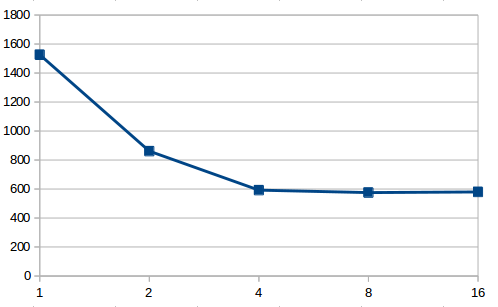
\includegraphics[width=0.7\linewidth]{res/threads}}
					\caption{Зависимость времени выполнения от количества потоков}
					\label{ris:threads}
				\end{figure}
				
				\begin{figure}[h]
					\center{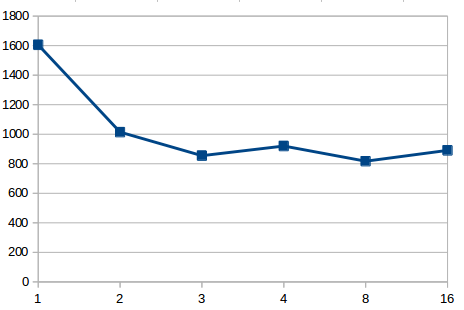
\includegraphics[width=0.7\linewidth]{res/mpi}}
					\caption{Зависимость времени выполнения от количества процессов}
					\label{ris:mpi}
				\end{figure}
				
				Как видно из результатов работы, при увеличении числа процессов 
				(потоков) до количества ядер позволяет уменьшить время выполнения программы (до 2 раз при достижении количества физических ядер и до 3 раз - логических), после чего две программы ведут себя несколько по разному. Программа, в которой используются потоки, 
				при задании количества потоков больше, чем количество ядер процессора 
				практически не меняет свои временные показатели (рисунок~\ref{ris:threads}). Программа, в которой использовалась технология MPI (рисунок~\ref{ris:mpi}), напротив, при задании количества процессов, большее, чем количество ядер, значительно ухудшила 
				свои показатели. Это, скорее всего, связано с тем, что передача 
				сообщений между процессами занимает значительное время.
				
				При количестве процессов больше, чем количество ядер происходит небольшой 
				скачек, что, вероятно, вызвано процедурой планирование (увеличивается СКО).
				При дальнейшем увеличении числа процессов СКО уменьшается, а так же уменьшается время выполнения программы.
				
			\section{Вывод}
			
				Целью данной лабораторной работы было показать увеличение 
				производительности при разбиение программы на несколько параллельно 
				работающих частей.
				
				В результате работы было опробованы две технологии распараллеливания 
				программы: pthreads и MPI. В результате, при оптимальных параметрах 
				каждая из технологий дала прирост в производительности примерно в 3 
				раз (при 4 рабочих потоках (процессах)), что является хорошим 
				результатом.
				
				Для синхронизации параллельной работы в Pthreads были использованы 
				мьютексы, а в MPI работа была организована при помощи создания главного 
				процесса,	который организует работу подчиненных процессов.
				
				При увеличении количества потоков (процессов) скорость выполнения 
				программы растет нелинейно из-за синхронизации потоков, а так же, 
				экспериментально было выявлено, что наилучшие показатели, как для 
				многопоточной, так и для MPI наилучшие показатели достигаются тогда, 
				когда количество потоков (процессов) равно количеству ядер в 
				компьютере. Так же стоит отметить, что при большом количестве потоков, 
				многопоточная программа практически не получает прироста 
				производительности. Программа, использующая технологию MPI, напротив, 
				значительно замедляется при большом количестве процессов, что 
				вызывается задержками при передачи сообщений.
				
				Для правильной оценки времени работы программы были произведены 
				многократные запуски (около 50 раз для каждого случая), что бы 
				исключить погрешности, например, вызванные процедурой планирования.
				
			\section{Листинги}

				\lstinputlisting[style={CppCodeStyle},caption={Параллельная 
				программа при помощи pthreads}]{../parallel/main.cpp}
			
				\lstinputlisting[style={CppCodeStyle},caption={Параллельная 
				программа при помощи MPI}]{../mpi/main.cpp}
			
	
				\begin{lstlisting}[language=bash,caption={bash version},texcl=true,
				frame=single,
				breaklines=true,
				extendedchars=\true]
#!/bin/bash

RDIR=`pwd`
TEST_DIR="$RDIR/TestFiles"
TEST_FILES="test3.txt"
REPORT_DIR="$RDIR/Reports"

# Количество повторений
let COUNTER_VAR=50

# Запуск задач
for i in $TEST_FILES ; do
    echo "Start thread programm for test file $i"
    $RDIR/progThread 4 $TEST_DIR/$i > $REPORT_DIR/"$i".result.thread
    echo "Start mpi programm for test file $i"
    mpirun -np 4 $RDIR/progMPI $TEST_DIR/$i > $REPORT_DIR/"$i".result.mpi
done

# Многократный запуск для последующего рассчета СКО и т.д.

TEST_FILE=test3.txt

# Подготовка
find -name *.repeate | xargs rm -f

# Параллельная программа с 1 потоком
#COUNTER=0

#echo "Start pthreads programm with 1 thread repeating..."
while [ $COUNTER -lt $COUNTER_VAR ] ; do
    $RDIR/progThread 1 $TEST_DIR/$TEST_FILE | head -n 1 >> $REPORT_DIR/result.threads.1.repeate
    let COUNTER=COUNTER+1
done
echo "Done"
echo ""

# Параллельная программа с 2 потоками
COUNTER=0

echo "Start pthreads programm with 2 thread repeating..."
while [ $COUNTER -lt $COUNTER_VAR ] ; do
    $RDIR/progThread 2 $TEST_DIR/$TEST_FILE | head -n 1 >> $REPORT_DIR/result.threads.2.repeate
    let COUNTER=COUNTER+1
done
echo "Done"
echo ""

# Параллельная программа с 4 потоками
COUNTER=0

echo "Start pthreads programm with 4 thread repeating..."
while [ $COUNTER -lt $COUNTER_VAR ] ; do
    $RDIR/progThread 4 $TEST_DIR/$TEST_FILE | head -n 1 >> $REPORT_DIR/result.threads.4.repeate
    let COUNTER=COUNTER+1
done
echo "Done"
echo ""

# Параллельная программа с 8 потоками
COUNTER=0

echo "Start pthreads programm with 8 thread repeating..."
while [ $COUNTER -lt $COUNTER_VAR ] ; do
    $RDIR/progThread 8 $TEST_DIR/$TEST_FILE | head -n 1 >> $REPORT_DIR/result.threads.8.repeate
    let COUNTER=COUNTER+1
done
echo "Done"
echo ""

# Параллельная программа с 16 потоками
COUNTER=0

echo "Start pthreads programm with 16 thread repeating..."
while [ $COUNTER -lt $COUNTER_VAR ] ; do
    $RDIR/progThread 16 $TEST_DIR/$TEST_FILE | head -n 1 >> $REPORT_DIR/result.threads.16.repeate
    let COUNTER=COUNTER+1
done
echo "Done"
echo ""

# MPI с 1 рабочим процессом
COUNTER=0

echo "Start MPI programm with 2 process repeating..."
while [ $COUNTER -lt $COUNTER_VAR ] ; do
    mpirun -np 2 $RDIR/progMPI $TEST_DIR/$TEST_FILE | head -n 1 >> $REPORT_DIR/result.mpi.1.repeate
    let COUNTER=COUNTER+1
done
echo "Done"
echo ""

# MPI с 2 рабочими процессами
COUNTER=0

echo "Start MPI programm with 3 process repeating..."
while [ $COUNTER -lt $COUNTER_VAR ] ; do
    mpirun -np 3 $RDIR/progMPI $TEST_DIR/$TEST_FILE | head -n 1 >> $REPORT_DIR/result.mpi.2.repeate
    let COUNTER=COUNTER+1
done
echo "Done"
echo ""

# MPI с 3 рабочими процессами
COUNTER=0

echo "Start MPI programm with 4 process repeating..."
while [ $COUNTER -lt $COUNTER_VAR ] ; do
    mpirun -np 4 $RDIR/progMPI $TEST_DIR/$TEST_FILE | head -n 1 >> $REPORT_DIR/result.mpi.3.repeate
    let COUNTER=COUNTER+1
done
echo "Done"
echo ""

# MPI с 4 рабочими процессами
COUNTER=0

echo "Start MPI programm with 5 process repeating..."
while [ $COUNTER -lt $COUNTER_VAR ] ; do
    mpirun -np 5 $RDIR/progMPI $TEST_DIR/$TEST_FILE | head -n 1 >> $REPORT_DIR/result.mpi.4.repeate
    let COUNTER=COUNTER+1
done
echo "Done"
echo ""

# MPI с 8 рабочими процессами
COUNTER=0

echo "Start MPI programm with 9 process repeating..."
while [ $COUNTER -lt $COUNTER_VAR ] ; do
    mpirun -np 9 $RDIR/progMPI $TEST_DIR/$TEST_FILE | head -n 1 >> $REPORT_DIR/result.mpi.8.repeate
    let COUNTER=COUNTER+1
done
echo "Done"
echo ""

# MPI с 16 рабочими процессами
COUNTER=0

echo "Start MPI programm with 17 process repeating..."
while [ $COUNTER -lt $COUNTER_VAR ] ; do
mpirun -np 17 $RDIR/progMPI $TEST_DIR/$TEST_FILE | head -n 1 >> $REPORT_DIR/result.mpi.16.repeate
let COUNTER=COUNTER+1
done
echo "Done"
echo ""

		\end{lstlisting}
\end{document}